\chapter{Navigation}
\label{chp:b5}

In this chapter, we focus on our trajectory planning and control algorithms.
The trajectory planner receives a primitive behavior mode, for our case, either
stop or cruise mode, along with a set of waypoints as a reference path and
delivers a safe, feasible trajectory consisting of another set of waypoints
each has a recommended speed to the control block. The conrol block executes
the trajectory by adjusting the steering angle to closely follow the waypoints
at recommended speeds.

\section{Trajectory Planning}

We build a cubic spline curve from the reference waypoints to represent the
reference path. In order to generate trajectories along the reference path, we
use frenet frame as in \cite{cite14, cite15}. Because the map of the
environment is not known a priori for our scenario, the reference paths are
either extracted from the lanes or predefined for a specific traffic sign. We
define normal trajectory $d(t)$ and tangential trajectory $s(t)$ to our
reference path $\vec{r}(s)$ as shown in Figure \ref{figure:frenet}. To use the
same convention as \cite{cite15}, we also let $d(t)$ and $s(t)$ be offset
pattern and distance pattern, respectively. While the offset pattern
corresponds to lateral dispacement, distance pattern corresponds to
longitudinal acceleration and deceleration. We combine the two by
Equation \eqref{eq:trajectory} to obtain a trajectory.

\begin{figure}[h]
  \centering
  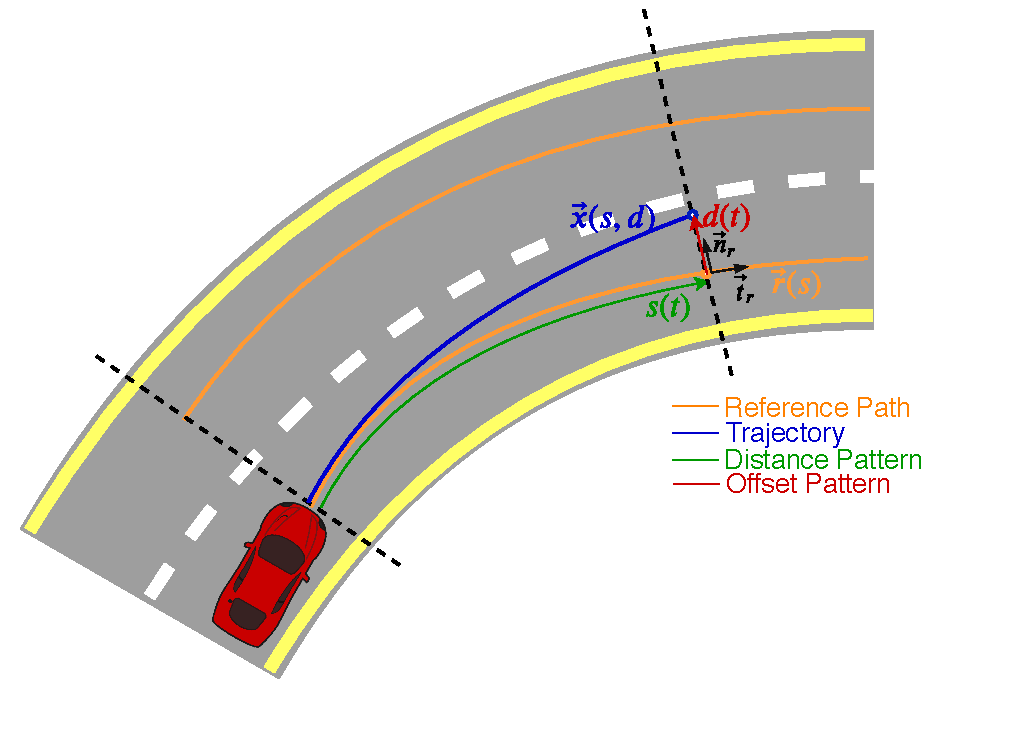
\includegraphics[width=1.0\textwidth]{figures/frenet-frame.pdf}
  \caption{Frenet frame based on the right reference path extracted
  from the right lane.}
  \label{figure:frenet}
\end{figure}

\begin{equation}
    \vec{x}(s(t), d(t)) = \vec{r}(s(t)) + d(t)\vec{n}_r(s(t))
\label{eq:trajectory}
\end{equation}

Offset and distance patterns are represented by 5-degree polynomials
in Equations \eqref{eq:dt} and \eqref{eq:st}.

\begin{equation}
    d(t) = a_0 + a_1t + a_2t^2 + a_3t^3 + a_4t^4 + a_5t^5
\label{eq:dt}
\end{equation}

\begin{equation}
    d(t) = a_0 + a_1t + a_2t^2 + a_3t^3 + a_4t^4 + a_5t^5
\label{eq:st}
\end{equation}

We generate a set of trajectories forward simulating various terminal
conditions for offset and distance patterns. $a_i$ and $b_i$ are calculated
using initial conditions $[d_0, \dot{d}_0, \ddot{d}_0]$, $[s_0, \dot{s}_0,
\ddot{s}_0]$ at $t_0$ and terminal conditions $[d_1, \dot{d}_1, \ddot{d}_1]$,
$[s_1, \dot{s}_1, \ddot{s}_1]$ at $t_1 = t_0 + \Delta T$, where $\Delta T$ is a
preview time in seconds. We use $4 < \Delta T < 6$ with $0.2$ second increments
for our offset and distance patterns. The offset pattern is defined as a
quintic function to control the lateral position.  The distance pattern is
defined using quartic and quintic function for cruise mode and stop mode,
respectively. In cruise mode, we don't pay attention to the terminal conditions
at longitudinal positions, but rather we focus on keeping the speed constant
around the speed profile set by the behavior planner; therefore, we set $b_5 =
0$. On the other hand, we specify a longitudinal position as a terminal
condition for the stop mode expecting the car to confortably slow down and
eventually stop at the specified position.

For the offset pattern, minimizing the lateral speed and accelaration leads to
a more confortable driving experience, so  we choose the terminal conditions
$[\Delta d, 0, 0]$ for the candidate trajectories, where $\Delta d = \{-0.1, 0,
1.0\}$ m. For cruise mode, we choose $[\dot{s}_1 + \Delta \dot{s}_1,
\ddot{s}_1]$, where $\Delta \dot{s}_1 = \{-0.1, 0, 0.1\}$ m/s and $\dot{s}_1$
is the target speed set by the behavior planner. For stop mode, we choose
$[s_1, 0, 0]$ terminal conditions, where $s_1$ is the stop position.

For all candidate trajectories, we apply a sanity check to see the candidate is
actually drivable. If there is an overlap between an obstacle grid of the
occupancy grid map and the car's bounding circle along a trajectory, we
conclude that the trajectory is not drivable. Non-drivable trajectories are
eliminated from the trajectory set. If no drivable trajectory is left, we set
the speed to zero until a valid trajectory is found again. Otherwise, the
trajectory with the minimum cost is selected among the surviving trajectories
as the best trajectory and forwarded to the controller for execution.
The cost function $C$ is defined in Equations \eqref{eq:cost1} -
\eqref{eq:cost3}.

\begin{equation}
    C = k_{path}C^i_{path} + k_dC_d + k_sC_s
\label{eq:cost1}
\end{equation}

\begin{equation}
    C_d = k_j\int_{t_0}^{t_1}\dddot{d}(t)dt + k_x\Delta T + k_y\Delta d^2
\label{eq:cost2}
\end{equation}

\begin{equation}
    C_s =
    \begin{cases}
        k_j\int_{t_0}^{t_1}\dddot{s}(t)dt + k_x\Delta T + k_y\Delta s^2,
        &\text{if stop mode;} \\
        k_j\int_{t_0}^{t_1}\dddot{s}(t)dt + k_x\Delta T + k_y\Delta \dot{s}^2,
        &\text{if cruise mode,}
    \end{cases}
\label{eq:cost3}
\end{equation}

where $C_d$ and $C_s$ are the costs from offset and distance patterns,
respectively. Both terms include integral of jerks, preview times, and
dispacement of terminal conditions. In multi-lane settings, $C^i_{path}$ is the
lane cost for \textit{i}th lane. For our scenario, we have only two lanes;
therefore, we assign a higher cost to the left lane so as to prevent the car
from occupying the left lane when the right lane is free as shown in Figure
\ref{figure:frenet-lanes}. In this way, the car automatically shifts to the
left lane when the right lane is blocked. Similarly, the car chooses the right
lane when it is available as it would be less costly than driving on the left
lane. We use $k_j = k_x = 0.1$ and $k_d = k_s = k_{path} = 1.0$ for our cost
evaluations.

\begin{figure}[h]
  \centering
  \begin{subfigure}[b]{1.0\linewidth}
      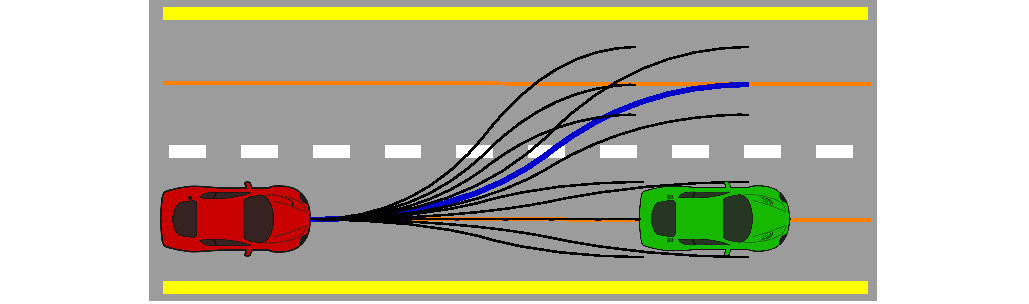
\includegraphics[width=\linewidth]{figures/frenet-shift-left-lane.pdf}
    \caption{}
  \end{subfigure}
  \begin{subfigure}[b]{1.0\linewidth}
      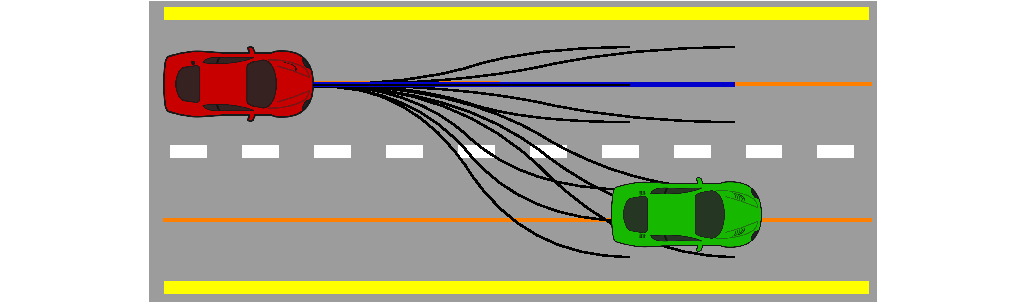
\includegraphics[width=\linewidth]{figures/frenet-keep-left-lane.pdf}
    \caption{}
  \end{subfigure}
  \begin{subfigure}[b]{1.0\linewidth}
      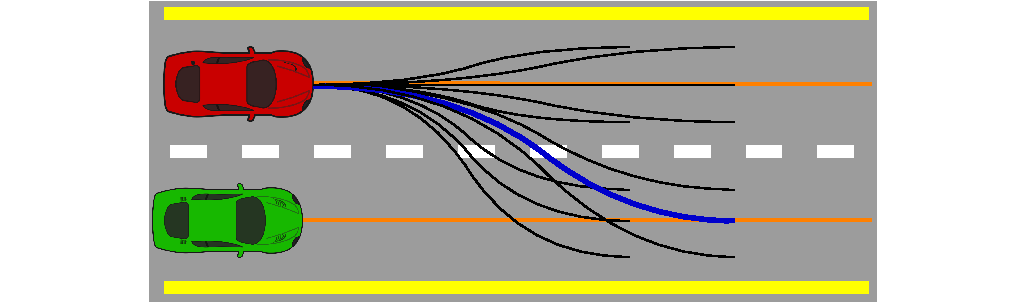
\includegraphics[width=\linewidth]{figures/frenet-shift-right-lane.pdf}
    \caption{}
  \end{subfigure}
  \caption{Example multi-lane driving scenario. The thick blue trajectory is
      the optimal trajectory for different cases. (a) The right lane is
      blocked, so the car attempts to change lane to the left for overtaking.
      (b) The right lane is still blocked, so the car keeps occupying the left
  lane. (c) Because the right lane is less costly when both lanes are
  available, the car shifts back to right lane.}
  \label{figure:frenet-lanes}
\end{figure}

\section{Trajectory Execution}

We use pure pursuit control algorithm to track the given optimal trajectory.
The algorithm relies on the nonholonomic constraints of the car. Let car
configuration be $\textbf{q} = [x y \theta]^T$, where $(x, y)$ is the position
and $\theta$ is the orientation of the car. Nonholonomic constraints satisfy
Equation \eqref{eq:nonholonomic}.

\begin{equation}
    \dot{x}\sin(\theta) - \dot{y}\cos(\theta) = 0
\label{eq:nonholonomic}
\end{equation}

such that longitudinal and lateral forces applied on the car tires are always
smaller than the maximum friction between the tires and the ground \cite{cite18}.
In other words we assume the car does not slip. With this constaints, we
estimate the steering angle in terms of turning radius $R$ and the wheelbase of
the car $L_b$ from Figure \ref{figure:steering} in Equation
\eqref{eq:steering}.

\begin{equation}
    \delta = \tan^{-1}(\frac{L_b}{R})
\label{eq:steering}
\end{equation}

\begin{figure}[h]
  \centering
  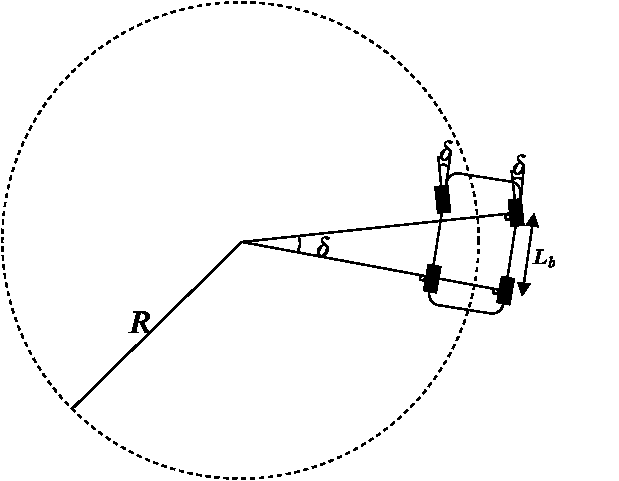
\includegraphics[width=0.8\textwidth]{figures/pure-pursuit-steering.pdf}
  \caption{Estimation of steering angle in terms of turning radius $R$ and
  wheelbase $L_b$.}
  \label{figure:steering}
\end{figure}

Given an optimal trajectory, we first find a point ahead of the car on the
trajectory such that the distance between the point and the car is the smallest
distance greater than a lookahead distance $L$. This is illustrated in Figure
\ref{figure:radius}.

\begin{figure}[h]
  \centering
  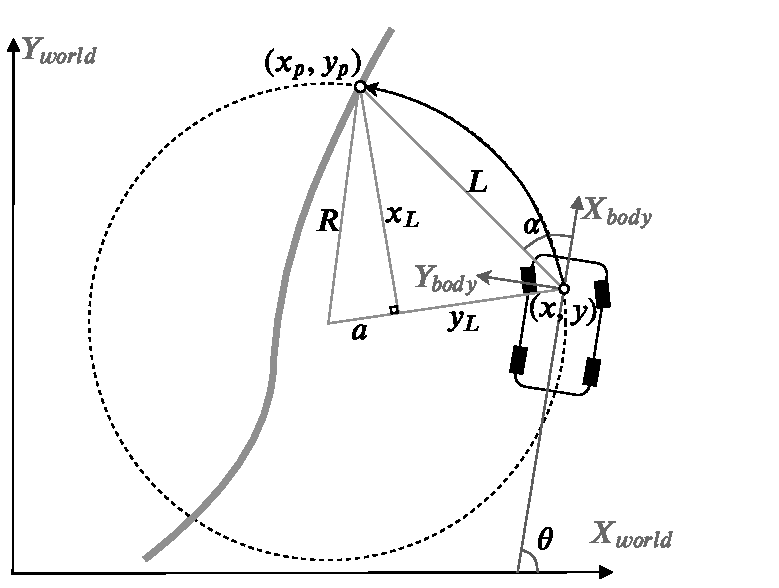
\includegraphics[width=0.8\textwidth]{figures/pure-pursuit-radius.pdf}
  \caption{Illustration of lookahead distance $L$ and feedback angle $\alpha$.}
  \label{figure:radius}
\end{figure}

From the figure, we write down the following equations:

\begin{equation}
    L^2 = x^2_L + y^2_L
\label{eq:radius1}
\end{equation}

\begin{equation}
    R^2 = a^2 + x^2_L
\label{eq:radius2}
\end{equation}

\begin{equation}
    R = a + y_L
\label{eq:radius3}
\end{equation}

\begin{equation}
    \sin{\alpha} = \frac{y_L}{L}
\label{eq:radius4}
\end{equation}

Combining \eqref{radius1}, \eqref{radius2}, and \eqref{radius3}, we obtain

\begin{equation}
    R = \frac{L^2}{2y_L}
\label{eq:radius5}
\end{equation}

Substituting \eqref{radius4} in \eqref{radius5}, we obtain and turning radius
$R$ in terms of feedback angle $\alpha$ and lookahead distance $L$.

\begin{equation}
    R = \frac{L}{2\sin{\alpha}}
\label{eq:radius6}
\end{equation}

Feedback angle $\alpha$ is computed by the car configuration $\textbf{q} = [x y
\theta]^T$ and the position of the lookahead point $(x_p, y_p)$ in the world
coordinates. Note that we take the midpoint of the front axle as the car
position in the world coordinates.

\begin{equation}
    \alpha = \tan^{-1}(\frac{y_p - y}{x_p - x}) - \theta
\label{eq:alpha}
\end{equation}

Finally, using \eqref{steering} and \eqref{radius6}, we derivate the steering
angle $\delta$ in terms of feedback angle $alpha$, constant wheelbase $L_b$,
and lookahead distance $L$.

\begin{equation}
    \delta = \tan^{-1}(\frac{2L_b\sin\alpha}{L})
\label{eq:delta}
\end{equation}

In order to tune the controller, we need to choose a lookahead distance $L$.
\cite{cite18} suggests $L = 2R_{min}$, where $R_{min} =
\frac{L_b}{\tan({\delta_{max})}}$. For our car, the max steering angle
$\delta_{max} = 0.34$ rads and the wheelbase $L_b = 0.25$ meters. Therefore, we
use $L = 1.4$. Figure \ref{figure:lookahead} illustrates the relation between
$R_{min}$ and $L$.


\begin{figure}[h]
  \centering
  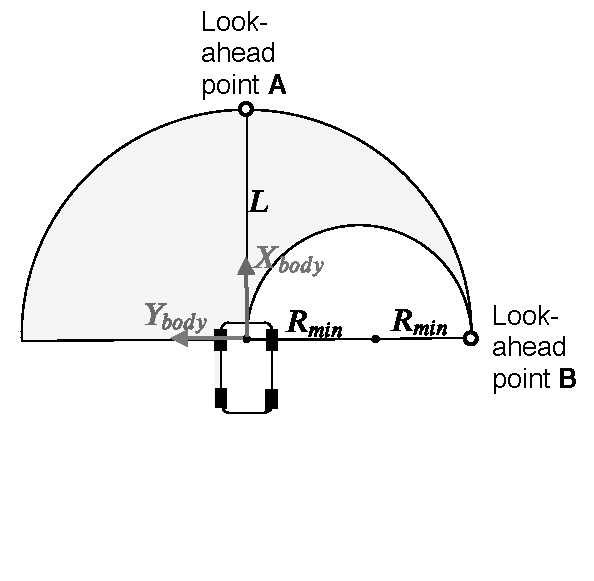
\includegraphics[width=0.8\textwidth]{figures/pure-pursuit-lookahead.pdf}
  \caption{Illustration of lookahead distance $L$ and minimum turning radius
  $R_{min}$ for tuning the pure pursuit controller.}
  \label{figure:lookahead}
\end{figure}

One problem with Equation \eqref{eq:delta} is that it does not account for the
speed. As the speed increases, steering angle $\delta$ becomes more sensitive
to the feedback angle $\alpha$ \cite{18}. WE address this problem by adding a
speed factor to lookahead distance $L$ in Equation \eqref{eq:lookahead}.

\begin{equation}
    L \leftarrow L + kv
\label{eq:lookahead}
\end{equation}

where $v$ is the recommended speed by the trajectory planner, $k$ is the look
forward gain. We use $k = 1$.

We compute a steering angle $\delta$ every time we receive an odometry message,
which is published at 15 Hz and contains the current car configuration
information.
